\documentclass[11pt]{article}

\usepackage{hyperref}  % links
\usepackage{graphicx}  % images
\usepackage{listings}  % code
\usepackage{authblk}  % author info
\usepackage{biblatex}  % bibliography
\usepackage{color}
\definecolor{green}{rgb}{0.0, 0.5, 0.0}
\lstdefinelanguage{JavaScript}{
  keywords={break, case, catch, continue, debugger, default, delete, do, 
  else, false, finally, for, function, if, in, instanceof, new, null, return, 
  switch, this, throw, true, try, typeof, var, void, while, with, let, const},
  morecomment=[l]{//},
  morecomment=[s]{/*}{*/},
  morestring=[b]',
  morestring=[b]",
  ndkeywords={class, export, boolean, throw, implements, import, this},
  keywordstyle=\color{blue},
  ndkeywordstyle=\color{blue},
  identifierstyle=\color{black},
  commentstyle=\color{green},
  stringstyle=\color{red},
  sensitive=true
}

\lstset{
   language=JavaScript,
   extendedchars=true,
   showstringspaces=false,
   showspaces=false,
   numbers=left,
   numbersep=5pt,
   tabsize=8,
   breaklines=true,
   showtabs=false,
   captionpos=b
}

\addbibresource{bib.bib}

% Preamble
\title{Angular, React or Vue.js: Which is Most Practical?}
\author{Brent Schaeffer}
\date{\today}

% Document body

\begin{document}

\maketitle

\begin{abstract}
    This paper is meant to take a look into three popular JavaScript based web frameworks that are common into today's industry:
    Angular, Vue.js, and React. The basis of this is to get a general idea of what each framework is and then comprare them to see
    if there is a "best" option out there.
\end{abstract}

\section{Web Frameworks}
What is a web framework and what is their purpose?
A majority of modern websites use JavaScript in some shape or form, to make the pages more
interactive and to handle functionality(Saks, Elar)\cite{saks2019javascript}. Traditionally in the past webpages were larger multi-page applications (MPAs)
that had to load different HTML documents whenever a user chagned pages or requested new content from the server.
This however is a relatively slow and time consuming option compared to the more modern day approach of single page application
(SPA). SPAs work in improving the time it takes to load an application by fetching the data from a server, 
then updating the current page contents with the fetched data, instead of loading a whole new document. 
This in turn also increases the quality of the users experience with the applications interface. Now this does not mean
that MPAs are not used today, they are, but working with web frameworks allows the reduction in the size of MPAs, better user experience,
and faster web applications. In other terms frameworks are designed to support and help developers develop web applications
in a more consistent and reliable way, as said by Elar Saks, "Frameworks dictate the application development workflow, reduce the development time and
possible errors". 

In the world of frameworks there are tons of available choices and the criteria to be considered one is somewhat open and can at times
be confused with libraries. A library generally consists of pre-written code, classes, procedures, scripts, configuration data, and more.
Mostly, it can be integrated in an existing project with ease and used to shorten development time. This is due to the fact that many 
issues concerning basic algorithms and functions have already been solved by another expert programmer in the community(Wohlgethan, Eric)\cite{wohlgethan2018supportingweb}.
It can be thought of in this manner, libraries are used to enhance a program or application, but on their own they cannot offer a complete 
stack of tools for development purposes. A simplified idea of this can be seen below in figure \ref{fig:1}.In comparison to libraries, 
frameworks indeed offer a complete stack of helpful functions and take responsibility for decisions that otherwise the developer
would have to make prior to actually writing the application’s code. This includes strategies for in-app routing of URL paths, 
state management, bundling and others. Furthermore, frameworks provide workflow improvements which include best practices
for basic development aspects like the overall structure of an application or generating boilerplate code. In a sense one can think of
frameworks as fully fledged libraries while there also exists other libraries that contain useful tools, but are not a complete 
set of tools to stand on their own. 

\begin{figure}[h]
    \centering
    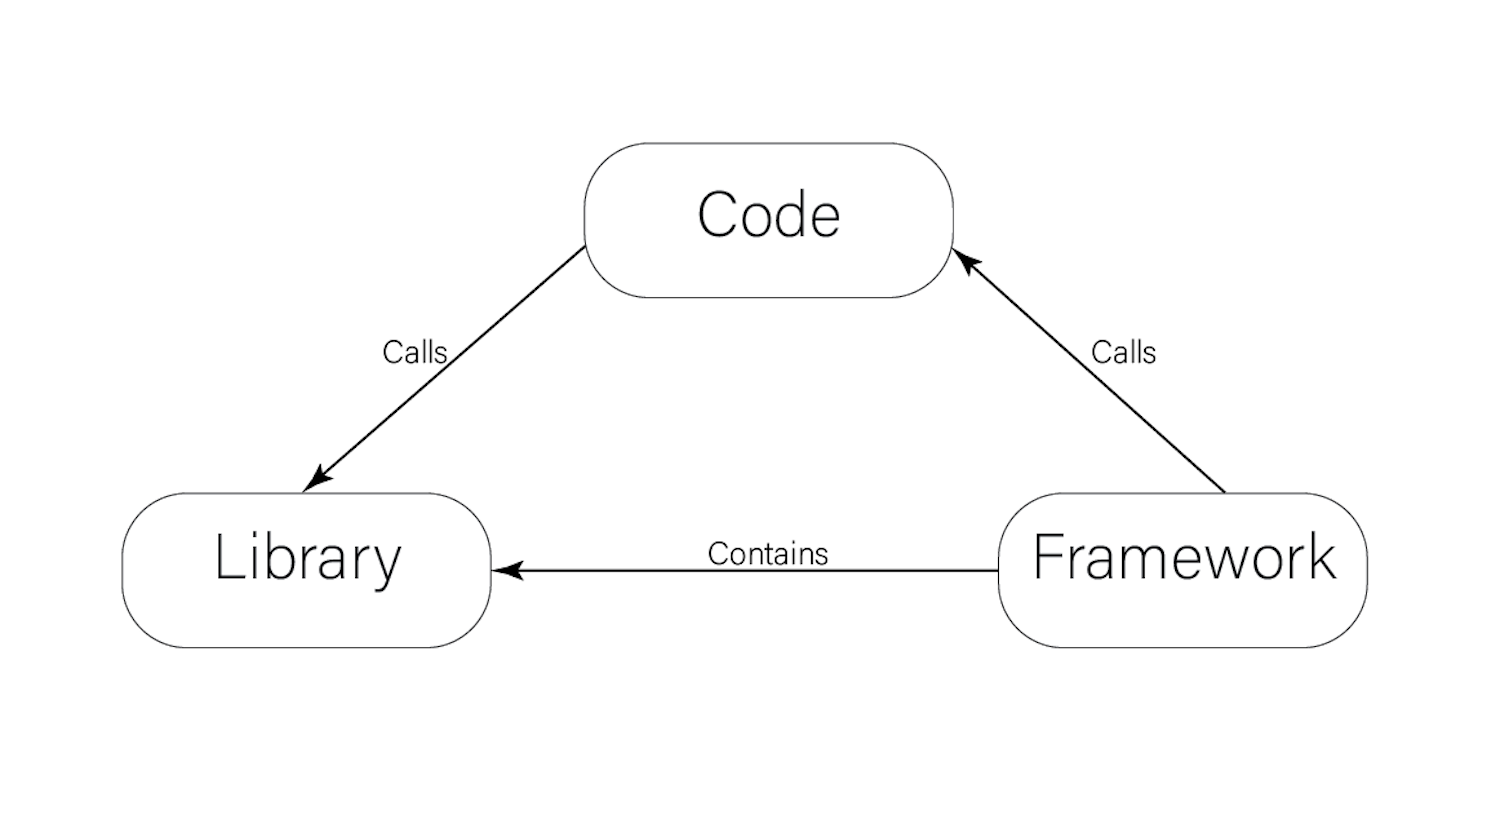
\includegraphics{flowchart}
    \caption{Libraries compared to frameworks}
    \label{fig:1}
\end{figure}    

\section{Angular} 
Angular was originally crated at Google by two employees Misko Harvey and Adam Abrons back in 2008. The first or original version
of Angular (now referred to as AngularJs) was completely developed in vanilla JavaScript as at the time MPAs were widely used and
browsers were not as powerful as they are today. Following the progression of Angular, in 2014 Angular 2 was announced and fully
released in 2016. Angular 2 was a complete re-imagining of the original released framework in two ways: AngularJs had an architecture
pattern that mainly focused on the use of scopes and controllers, while Angular 2's architecture focused completely on components, and 
the notably largest change was the use of TypeScript. Components follow the Mode-View-Controller (MVC) pattern as each component uses the 
same architecture. Think of it this way the components code represents the controller and the HTML code plus CSS represent the view.

\subsection{TypeScript}
    TypeScript is a superset of JavaScript. Unlike JavaScript, TypeScript has to be transcompiled into
plain JavaScript in order for it be used. The advantage of TypeScript is one has access to all the functionality of JavaScript like lambdas, 
loops, and most importantly decorators, which are very important in Angular. TypeScript has become popular to use in the programming community
due to having strong typing of code. The similarities and difference can be seen in the example: Listing \ref{lst1}

\begin{lstlisting}[caption={JavaScript vs TypeScript},label={lst1}]
//JavaScript
const message = 'hello world';
function greet(name) {
    return `Hello, ${name}`;}
let myAdd1 = function (x, y) { return x + y; };
let myAdd2 = function (x, y) { return x + y; };

console.log(message); //Returns: hello world
console.log(myAdd1(12, 12)); //Returns: 24
console.log(myAdd1("hello", 15)); //Returns hello15

//TypeScript
const message: string = 'hello world';
function greet(name: string) {
    return `Hello, ${name}`}
let myAdd1 = function(x: number, y: number): number { return x + y; };
let myAdd2: (x: number, y: number) => number =
    function (x: number, y: number): number { return x + y; };
  
console.log(message); //Returns: hello world
console.log(myAdd1(12, 12)) //Returns: 24    
console.log(myAdd1("hello", 15)) //Raises Error
\end{lstlisting}

At a quick glance they almost seem the same but there are notable difference between the two. One of course is the strong typing, for example with the const message. 
In JavaScript one doesn't need to declare that it's a string, but in TypeScript you have to. This can also be seen in the myAdd1 function where one can declare that a 
number should be returned from the function and nothing else. Finally, when trying to call the function myAdd1 if a number is not passed to the function an error is 
raised because it has been declared that a number must be passed into the function. One last importance to note is how the myAdd1 and myAdd2 look in JavaScript and TypeScript, 
one can see that in JavaScript they both look the same, but in TypeScript it's more explicit on what should be passed and returned from the function.

\subsection{Angular Components}
Angular, like many other frameworks, is component-based. This means that components are the main building blocks. They can display information, render templates
and perform actions on data(Maximilian Schwarzmüller)\cite{ReactvsA7:online}. In theory components are comprised in three parts or document: the HTML file for the 
template, a CSS file for adding styles and of course a TypeScript file acting as the controller. Following this structure allows for a clean organized project and 
code. As said before Angular components are structured in a hierarchical manner meaning data can be passed between parent and child nodes, two or more child nodes,
and even between non linked nodes. Angular comes with a wide variety of components, but it also allows for custom ones to be made by a developer, for example 
Listing \ref{lst3} is a simple building of a new component.
\begin{lstlisting}[caption={Simple Angular component}, label={lst3}]
import { Component } from "@angular/core";
@Component({
  selector: "my-component",
  template: "Hello Angular"
})
class MyComponent {
}
\end{lstlisting}

If used in HTML (\textless my-component\textgreater \textless /my-component \textgreater) and run in a browser your window would simply show up with 'Hello Angular' on the top left corner of your screen. 
This is just a simple example of creating your own Angular component and there is a bit more to the process, but this captures it in essence. Like 
other frameworks components can be built and reused over and over again if needed.

\section{React}
React.js or more commonly known just as React is a JavaScipt library developed by Facebook and its community to aid developers in the creation
of web applications. It's initial release was in May 2013 and since then has become one of the most popular tools for application developers. React uses 
JavaScript XML (JSX), which is simply a syntax extension of JavaScript. JSX is an XML/HTML-like syntax used by React that extends ECMAScript so that XML/HTML-like text 
can co-exist with JavaScript/React code. The syntax is intended to be used by preprocessors (i.e., transpilers like Babel) to transform HTML-like text found in 
JavaScript files into standard JavaScript objects that a engine will parse\cite{JSXWhatI92:online}. React like Angular is component based, but the architecture is vastly 
different between the two. React has what is called a Virtual Document Object Model (VDOM) that handles making changes in the browsers DOM. In essences the VDOM
holds a replica of the UI in its memory and the browser DOM is then connected through a JS library, which in this case is React. This in turn takes attribute 
and event handing and makes the updating of the DOM automated instead of being manual. 

\subsection{JSX}
To show how JSX works we can make a quick navigation bar for a fake application that would be used to route to different parts of the app. One can see the JSX code here (Listing \ref{lst5}) 
written withinin JavaScript. Now the code is not able to be run just as it is, it has to then be transcompiled, React recommends using Babel, but of course there are others out there that 
can be used. Babel then turns the code into readable JavaScript (Listing \ref{lst6}) that can now be parsed.

\begin{lstlisting}[caption={JSX code sample}, label={lst5}]
const nav = (
    <ul id="nav">
      <li><a href="#">Home</a></li>
      <li><a href="#">About</a></li>
    </ul>
);
\end{lstlisting}

\begin{lstlisting}[caption={Transcompiled JSX}, label={lst6}]
const nav = 
    React.createElement("ul",{ id: "nav" },
    React.createElement("li",null,
       React.createElement("a",{ href: "#" },"Home")
    ),
    React.createElement("li",null,
       React.createElement("a",{ href: "#" },"About")
    )
 );
\end{lstlisting}
Now of course if a programmer wanted to they could originally write the code so that it wouldn't have to be transcompiled, but as you can see from the sample it is definitely less
time consuming, cleaner, and frankly more easily understandable using JSX. 

\subsection{React Components}
Like the others React is based on components. As said earlier the focus of React is to mutate or change the state of an appplication
using the VDOM and real DOM that is then displayed in the browser. There are two possible ways to write components in React: Components as \textbf{Functions} or 
as \textbf{Classes}. Components as Functions act normally as functions would, in which they return exactly one ReactElement. In this case the function name also paralles 
and is the name for the component. However component functions have many limitations. On the other hand components as classes are much more powerful \ref{lst7}. In general the developers of React recommend using function components more so than
class ones. This will in turn provide efficient code that can be used over and over again. In reality classes are used more to handle and delegate functionality.
\begin{lstlisting}[caption={Simple React component}, label={lst7}]
    class Hello extends React.Component {  
        render() {  
            return <h1>Hello world!</h1>;  
        }  
    }
    ReactDOM.render(  
        <Hello />,   
        document.querySelector("#app")
    );
\end{lstlisting}

\begin{lstlisting}[language=HTML, caption={React HTML example}, label={lst8}]
<!DOCTYPE html>
<html lang= "en" >
<body>  
    <div id="app">
        <!-- Add message here  -->
    </div>
    </body>  
</html>
\end{lstlisting}
In the case of these two examples the code executed in Listing \ref{lst7} targets the \textbf{div} element in Listing \ref{lst8} by querrying its id, and 
then it procedes to return and place the h1 with text: \textbf{Hello world!} inside of the targeted div. If this was rendred in a browser there would simply
be a header in the top left corner that says Hello world!

\section{Vue.js}

Vue.js was created by Evan You, who before was an employee of Google where he worked extensivly with AngularJs. The first initial stable release
came in October 2015. Vue is a progressive framework for building user interfaces. Unlike other monolithic frameworks, Vue is 
designed from the ground up to be incrementally adoptable. The core library is focused on the view layer only, and is easy to pick up and integrate with other 
libraries or existing projects\cite{Vuejs0:online}. The architecture of vue is comprised of reusable components known as \textbf{Vue Instances}. What sets Vue apart from the other frameworks is that it is developed by the open source
community and not a large company like Google or Facebook. Vue itself started as a side project by its creator Evan You, until he decided to leave Google and 
focus full time on his project.

\subsection{Vue Components}
Vue is component based as seen in listing \ref{lst9} All Vue components are also instances, on the creation of a Vue instance, all properties that can be found in its data object are added to the frameworks 
reactivitysystem. With that said if the template tag is called in an HTML document then you would see the resuling message of "A dog has 4 legs ..."
\begin{lstlisting}[caption={Vue component}, label={lst9}]
Vue.component('dog-info', {
    data: function() {
        return {
            legs: 4,
            eyes: 2
        }
    },
    template: '<h1>A dog has {{ legs }} legs and {{ eyes }} eyes.</h1>' })
\end{lstlisting}
When is comes to data binding vue has two options in which you can bind data between the model and view. One of the common ways is using v-bind, this can be seen in listing \ref{lst10}. In this case there is a vue
instance (Listing \ref{lst11}) which is targeting the div element with id app. First off you can notice the special stynax \{\{ \}\} that is used to fill the div element with the Vue instance message. Which in the 
Broswer would show the message that says "Hell CS330". Second, the v-bind then binds the title of the HTML element to the data title in the vue instance, which if the mouse hovered over the message it would tell 
the user when the page was loaded. 
\begin{lstlisting}[language=HTML, caption={HTML Code for Vue Example}, label={lst10}]
<!DOCTYPE html>
<html lang= "en" >
<body>
    <div id="app" v-bind:title="title">
        {{ message }}
    </div>
    <script src="https://cdn.jsdelivr.net/npm/vue/dist/vue.js"></script>
    <script src="script.js"></script>
</body>
</html>
\end{lstlisting}

\begin{lstlisting}[caption={Vue.js example}, label={lst11}]
new Vue({
    el: "#app",
    data: {
        message: "Hello CS330",
        title: "This page has been loaded on " + new Date().toLocaleString()
    }
});  
\end{lstlisting}

\section{Learnability}
\subsection{Angular}
Angular is by far the hardest of the three frameworks to learn initialy, if one has no previous knowledge or experience with it. This can be attributed to not only learning how Angular works, but having to learn a new language,
TypeScript. Now TypeScript is very similar to JavaScript and if one knows JS then TS shoudn't be too bad to learn. The other factor is on top of learning TypeScript the syntax of Angular is by far also the most rigurous to 
learn

\subsection{React}
React is not as big of a learning curve because the use of JSX is not hard to learn especially for anyone who has previous experience using HTML and JavaScript. JSX is not too hard to understand and can feel 
very comfortable to new users.

\subsection{Vue.js}
Vue.js by far has the easiest or initial starting learning curve and this can be attributed to a couple reasons. All of Vue's syntax is a valid form of HTML and can look very similar to what is already built into classic HTML,
 JavaScript and CSS.

\subsection{Result}
If only one option had to be picked I would say Vue.js would win when it comes to the ability to learn it initially, but since that's not the case I would call it more or less a tie between Vue.js and React as they both have features
that make the frameworks easier for newer users to learn and become well versed in them

\section{Performance}
In the search to see if one framework performed better than the other I found a project by Stefan Krause \cite{Interact81:online} where one could compare many different kinds of frameworks and their Performance doing tasks from creating 
a table with 1,000 rows to replacing the data in the rows and other instances of changing content of the rows, as well as how long it takes for a frameworks scripts and other conect to lead. In general when comparing Angular, Vue and 
React they are have  similar bench marks when it comes to the amount of time they take to perform these actions. Of course the data is also a mean of these tests being run multiple times. In all the metrics that were measured Vue 
actually was the quickest in performance, but they are all close and similar. This must also be taken with a grain of salt as run time also doesn't determine other aspects of frameworks in their strengths and weaknesses.

\section{Popularity}
Thre are two ways to look at these frameworks popularity in general and popularity in the workplace. It is hard to find exactly which is more popular, but many use the stars that are given on GitHub repositories to guage the popularity.
A sudden shift in the number of stars of Vue occurred in mid-2016 and, recently, Vue has been up there with React among the most popular frameworks\cite{Angularv42:online}. Now it makes sense why Vue has jumped in popularity as it is
not too diffuclt to pick up for someone new. Now the second way to measure popularity is the need for each framework in the workplace. For all the different websites that advertise jobs like LinkedIn and Indeed, an overwhelming amount
of the jobs were looking for people with experience in Angular over the other two. 

\section{Conclusion}
Overall each framework has its pros and cons, but it is impossible to flat out say which one is best put a stamp on it and call it good, no. In most cases it varies on what the user wants to get out of it. In the case of Vue.js because 
it has a learning curve that is not too hard and one can pick it up quickly I would recommend Vue.js in an educational setting as a good precursor for learning about frameworks and then if one wants they can move on to something else 
like React or Angular. Now when it comes to the working and business world I would says React and Angular have a stronger foot hold in the community as in companies expecting an employee to either know these frameworks or having to use it.
In reality it all depends also on the company, what work is being done and many other facts, but overall React and Angular have a stronger base. If there is one framework that would be best to use thought it would be Angular. Although 
the learning curve at the start may be harder the marketability of this skill is high and wanted by many companies out in the workplace. 


\printbibliography

\end{document}